\documentclass[conference]{Plantilla_LATEX/IEEEtran}
\IEEEoverridecommandlockouts

\usepackage[utf8]{inputenc}
\usepackage[T1]{fontenc}
\usepackage[spanish,es-tabla]{babel}
\usepackage{cite}
\usepackage{amsmath,amssymb,amsfonts}
\usepackage{graphicx}
\usepackage{textcomp}
\usepackage{xcolor}
\usepackage{booktabs}
\usepackage{siunitx}
\usepackage{url}

\graphicspath{{images/}{diagrams/}{Plantilla_LATEX/}}
\sisetup{
  output-decimal-marker = {.},
  separate-uncertainty = true,
  per-mode = symbol
}

\def\BibTeX{{\rm B\kern-.05em{\sc i\kern-.025em b}\kern-.08em
    T\kern-.1667em\lower.7ex\hbox{E}\kern-.125emX}}


\begin{document}

\title{Título de la práctica de laboratorio}

\author{
\IEEEauthorblockN{1\textsuperscript{ro} Apellidos, Nombres}
\IEEEauthorblockA{\textit{Carrera} \\
\textit{Universidad Centroamericana José Simeón Cañas} \\
Antiguo Cuscatlán, El Salvador \\
correo@uca.edu.sv}
\and
\IEEEauthorblockN{2\textsuperscript{do} Apellidos, Nombres}
\IEEEauthorblockA{\textit{Carrera} \\
\textit{Universidad Centroamericana José Simeón Cañas} \\
Antiguo Cuscatlán, El Salvador \\
correo@uca.edu.sv}
}

\maketitle

\begin{abstract}
Se estudiaron experimentalmente los principios de Arquímedes, continuidad y Torricelli mediante dos montajes de laboratorio. En la primera parte, se sumergió progresivamente una varilla en agua y se registraron, para diez longitudes sumergidas, la lectura de una balanza de brazo triple y su diferencia respecto a una lectura de referencia. La relación lineal entre ambas variables permitió determinar una densidad experimental del agua de $\SI{0.991}{\gram\per\cubic\centi\meter}\pm\SI{0.012}{\gram\per\cubic\centi\meter}$, con un error porcentual de $0.86\%$ y un coeficiente de determinación de $R^2=0.9930$. Se consideraron incertidumbres de $\pm\SI{0.05}{\gram}$ para la balanza, $\pm\SI{0.10}{\gram}$ para la diferencia entre lecturas y $\pm\SI{0.05}{\centi\meter}$ para las mediciones de longitud y diámetro. En la segunda parte, se midieron los tiempos de vaciado de un recipiente de Torricelli para alturas iniciales de $\SI{10}{\centi\meter}$, $\SI{8}{\centi\meter}$, $\SI{6}{\centi\meter}$, $\SI{4}{\centi\meter}$ y $\SI{2}{\centi\meter}$. El ajuste experimental fue $t=88.72h^{0.651}$, con $R^2=0.9806$, y los errores porcentuales respecto al modelo teórico variaron entre $5.73\%$ y $22.48\%$, con un promedio de $14.65\%$. Los resultados respaldaron la proporcionalidad entre el volumen desplazado y la inmersión, así como la dependencia sublineal del tiempo de vaciado con la altura inicial, aunque evidenciaron desviaciones respecto a las condiciones ideales.
\end{abstract}

\begin{IEEEkeywords}
palabra clave 1, palabra clave 2, palabra clave 3, palabra clave 4
\end{IEEEkeywords}

\section{Marco teórico}

\subsection{Principio de Arquímedes}

El principio de Arquímedes establece que un cuerpo sumergido total o parcialmente en un fluido experimenta una fuerza de empuje vertical hacia arriba, cuya magnitud es igual al peso del fluido desplazado \cite{serway2018,young2018}:

\begin{equation}
    E = \rho_f V_f g,
    \label{eq:empuje}
\end{equation}

donde $E$ es el empuje, $\rho_f$ es la densidad del fluido, $V_f$ es el volumen de fluido desplazado y $g$ es la aceleración de la gravedad.

En el experimento, una varilla se sumergió progresivamente en un beaker con agua colocado sobre una balanza. El aumento de la lectura de la balanza se atribuyó a la fuerza de reacción, igual y opuesta al empuje ejercido sobre la varilla, de acuerdo con la tercera ley de Newton.

Si la varilla posee un área transversal constante $A$, el volumen sumergido es $V_f=AL$. Por consiguiente, la diferencia de masa registrada por la balanza puede expresarse como

\begin{equation}
    \Delta m = (\rho_f A)L,
    \label{eq:deltam}
\end{equation}

donde $L$ es la longitud sumergida. La relación entre $\Delta m$ y $L$ es lineal, por lo que la pendiente $k$ del ajuste satisface $k=\rho_f A$. La densidad experimental del fluido se obtiene entonces mediante

\begin{equation}
    \rho_f = \frac{k}{A}.
    \label{eq:densidad}
\end{equation}

Para evaluar la consistencia del modelo, el intercepto del ajuste debe ser cercano a cero, pues un valor apreciable podría indicar la presencia de efectos sistemáticos o una lectura de referencia inadecuada.

\subsection{Ecuación de continuidad y teorema de Torricelli}

El vaciado de un recipiente con agua se describe mediante la ecuación de continuidad y el teorema de Torricelli. Para un fluido incompresible, la conservación del caudal entre el recipiente y el orificio de salida se expresa como

\begin{equation}
    A_1v_1=A_2v_2,
    \label{eq:continuidad}
\end{equation}

donde $A_1$ y $v_1$ son el área y la velocidad en el orificio, mientras que $A_2$ y $v_2$ corresponden al área y la velocidad de descenso del nivel en el recipiente. Esta relación representa la conservación de la masa del fluido \cite{young2018}.

El teorema de Torricelli, obtenido a partir de la ecuación de Bernoulli para un recipiente abierto a la atmósfera, permite calcular la velocidad de salida del agua por el orificio:

\begin{equation}
    v_1=\sqrt{2gh},
    \label{eq:torricelli}
\end{equation}

donde $h$ es la altura del nivel del agua medida desde el centro del orificio. Al combinar las ecuaciones de continuidad y de Torricelli, el tiempo teórico de vaciado puede escribirse en términos de áreas o diámetros como

\begin{equation}
    t_v=\left(\frac{A_2}{A_1}\right)\sqrt{\frac{2h}{g}}
    =\left(\frac{d_2}{d_1}\right)^2\sqrt{\frac{2h}{g}},
    \label{eq:tiempo_vaciado}
\end{equation}

donde $d_1$ es el diámetro del orificio y $d_2$ es el diámetro del recipiente. Esta expresión permite comparar el tiempo teórico de vaciado con el tiempo medido experimentalmente.

\subsection{Justificación del modelo experimental}

La determinación del empuje mediante la varilla y la balanza permite evaluar la relación entre el volumen de fluido desplazado y la lectura de la balanza. Debido a que el área transversal de la varilla se mantiene constante, se espera que la diferencia de masa aumente proporcionalmente con la longitud sumergida.

El experimento de vaciado permite estudiar la dependencia del tiempo necesario para vaciar el recipiente con respecto a la altura inicial del agua. Las mediciones de $h$ y $t$, junto con los diámetros $d_1$ y $d_2$, permiten comparar el comportamiento observado con el tiempo teórico obtenido mediante las ecuaciones de continuidad y de Torricelli.

\section{Metodología}

\subsection{Determinación experimental de la densidad mediante el principio de Arquímedes}

Para estudiar el empuje ejercido por el agua sobre una varilla parcialmente sumergida, se utilizó una balanza de brazo triple, un beaker de \SI{500}{\milli\liter} con agua, una varilla, soportes, una regla y un pie de rey. La balanza presentó una incertidumbre de $\pm\SI{0.05}{\gram}$; la regla y el pie de rey presentaron incertidumbres de $\pm\SI{0.05}{\centi\meter}$.

Inicialmente, se colocó el beaker con agua sobre la balanza y se equilibró el sistema sin sumergir la varilla. Esta lectura se tomó como referencia para la medición posterior de las variaciones de masa aparente. Luego, se fijó la varilla mediante los soportes y se sumergió progresivamente en el agua, comenzando con una longitud aproximada de \SI{1}{\centi\meter}. Para cada posición se midieron y registraron la longitud sumergida $L$, la lectura de la balanza y la \textit{Diferencia} entre dicha lectura y la lectura de referencia. La incertidumbre de la lectura de la balanza fue $\pm\SI{0.05}{\gram}$ y la incertidumbre de la \textit{Diferencia} fue $\pm\SI{0.10}{\gram}$. Se efectuaron diez mediciones correspondientes a diferentes valores de longitud sumergida $L$, procurando mantener el montaje estable y evitar el contacto de la varilla con las paredes o el fondo del beaker.

Una vez completadas las mediciones, se retiró la varilla y se determinó su diámetro con el pie de rey, cuya incertidumbre fue $\pm\SI{0.05}{\centi\meter}$. A partir de esta dimensión se obtuvo el área transversal de la varilla. Los datos quedaron organizados para su posterior representación gráfica de la diferencia de lectura en función de $L$; el procesamiento y la interpretación de dicha gráfica se presentan en la sección de análisis.

El esquema correspondiente debe mostrar la balanza con el beaker apoyado sobre su plataforma, la varilla suspendida mediante los soportes, la longitud sumergida $L$ y el instrumento utilizado para medir el diámetro. Se sugiere el pie de figura: ``Figura 1. Montaje experimental utilizado para medir el empuje sobre una varilla parcialmente sumergida.''

\subsection{Estudio del vaciado de un recipiente mediante continuidad y Torricelli}

Para estudiar el vaciado del recipiente se utilizó un recipiente de Torricelli con un orificio lateral, una regla y un cronómetro. Se midieron inicialmente el diámetro del orificio $d_1$ y el diámetro del recipiente $d_2$ con un pie de rey, cuya incertidumbre fue $\pm\SI{0.05}{\centi\meter}$. La regla se empleó para determinar la altura $h$ del nivel del agua respecto al centro del orificio, con una incertidumbre de $\pm\SI{0.05}{\centi\meter}$.

El recipiente se llenó inicialmente hasta alcanzar $h=\SI{10}{\centi\meter}$, manteniendo el orificio tapado durante el llenado. Al alcanzar la altura establecida, se retiró la obstrucción y se inició simultáneamente el cronómetro cuando comenzó la salida del agua. El cronómetro se detuvo cuando el flujo dejó de salir por el orificio y se registró el tiempo experimental de vaciado $t$. El procedimiento se repitió para cinco alturas iniciales: $h=\SI{10}{\centi\meter}$, $\SI{8}{\centi\meter}$, $\SI{6}{\centi\meter}$, $\SI{4}{\centi\meter}$ y $\SI{2}{\centi\meter}$. En cada repetición se verificó la altura con la regla y se mantuvieron las mismas condiciones geométricas del recipiente y del orificio. Los tiempos teóricos y los errores porcentuales se calcularon posteriormente y se reservaron para la sección de análisis.

El esquema de esta parte debe representar el recipiente de Torricelli, el orificio lateral, los diámetros $d_1$ y $d_2$, la regla junto al recipiente, la altura $h$ medida desde el centro del orificio y la trayectoria de salida del agua. Se sugiere el pie de figura: ``Figura 2. Montaje experimental utilizado para estudiar el vaciado de un recipiente mediante continuidad y el teorema de Torricelli.''

\section{Análisis}

\subsection{Determinación de la densidad del fluido mediante el principio de Arquímedes}

Para determinar experimentalmente la densidad del agua se midió la diferencia 
en la lectura de la balanza al sumergir gradualmente una varilla. 

De acuerdo con el principio de Arquímedes, el empuje ejercido por el fluido sobre 
el cuerpo es igual al peso del fluido desplazado \cite{young2018}:

\begin{equation}
E = \rho_f V_f g.
\end{equation}

Debido a la tercera ley de Newton, este empuje produce una variación en la lectura de la balanza. 
Por lo tanto, la diferencia de masa registrada puede relacionarse con 
el volumen de fluido desplazado mediante 

\begin{equation}
\Delta m = \rho_f V_f.
\end{equation}

Como la varilla posee una sección transversal constante, el volumen sumergido se expresa como

\begin{equation}
V_f = AL
\end{equation}

donde $A$ es el área transversal de la varilla y $L$ es la longitud sumergida. 
De esta manera se obtiene la relación lineal

\begin{equation}
\Delta m = \rho_f A L.
\end{equation}

Por tanto, al representar la diferencia de masa $\Delta m$ en función de la longitud sumergida $L$, 
la pendiente del ajuste lineal está dada por

\begin{equation}
k = \rho_f A,
\end{equation}

de donde la densidad experimental puede calcularse mediante

\begin{equation}
\rho_f = \frac{k}{A}.
\end{equation}

Los datos experimentales obtenidos se presentan en la Tabla~\ref{tab:datos_arq}.

\begin{table}[htbp]
\centering
\caption{Mediciones de la longitud sumergida y diferencia de masa registrada por la balanza.}
\label{tab:datos_arq}
\begin{tabular}{ccc}
\hline
$L$ (cm) & Lectura de balanza (g) & $\Delta m$ (g) \\
\hline
$0.00$ & $435.50 \pm 0.05$ & $0.00 \pm 0.10$ \\
$1.00 \pm 0.05$ & $437.00 \pm 0.05$ & $1.50 \pm 0.10$ \\
$2.00 \pm 0.05$ & $438.60 \pm 0.05$ & $3.10 \pm 0.10$ \\
$3.00 \pm 0.05$ & $439.80 \pm 0.05$ & $4.30 \pm 0.10$ \\
$4.00 \pm 0.05$ & $440.00 \pm 0.05$ & $4.50 \pm 0.10$ \\
$5.00 \pm 0.05$ & $442.20 \pm 0.05$ & $6.70 \pm 0.10$ \\
$6.00 \pm 0.05$ & $443.20 \pm 0.05$ & $7.70 \pm 0.10$ \\
$7.00 \pm 0.05$ & $444.40 \pm 0.05$ & $8.90 \pm 0.10$ \\
$8.00 \pm 0.05$ & $446.00 \pm 0.05$ & $10.50 \pm 0.10$ \\
$9.00 \pm 0.05$ & $447.20 \pm 0.05$ & $11.70 \pm 0.10$ \\
$10.00 \pm 0.05$ & $448.50 \pm 0.05$ & $13.00 \pm 0.10$ \\
\hline
\end{tabular}
\end{table}

El diámetro de la varilla se midió como

\begin{equation}
D=(1.275\,\mathrm{cm}\pm0.05\,\mathrm{mm}).
\end{equation}

A partir de este valor, el área transversal se calculó mediante

\begin{equation}
A=\frac{\pi D^2}{4},
\end{equation}

obteniéndose

\begin{equation}
A=(1.277\pm0.100)\,\mathrm{cm^2}.
\end{equation}

La incertidumbre del área se obtuvo mediante propagación de incertidumbres, siguiendo el procedimiento descrito en \cite{taylor1997}:

\begin{equation}
\frac{\Delta A}{A}
=
2\frac{\Delta D}{D}.
\end{equation}

La gráfica de la diferencia de masa en función de la longitud sumergida se muestra en la Fig.~\ref{fig:ajuste_arq}.
El ajuste lineal obtenido fue

\begin{equation}
\Delta m =
(1.266\pm0.011)L
+
(0.227\pm0.068),
\end{equation}

con un coeficiente de determinación

\begin{equation}
R^2=0.9930.
\end{equation}


\begin{figure}[htbp]
\centering
\begin{tikzpicture}
\begin{axis}[
    width=\columnwidth,
    height=0.68\columnwidth,
    xlabel={Longitud sumergida, $L$ (cm)},
    ylabel={Diferencia de masa, $\Delta m$ (g)},
    xmin=0, xmax=10.5,
    ymin=0, ymax=14,
    grid=major,
    legend style={font=\scriptsize, at={(0.03,0.97)}, anchor=north west},
    tick label style={font=\scriptsize},
    label style={font=\scriptsize}
]
\addplot+[
    only marks,
    mark=*,
    mark size=1.4pt,
    error bars/.cd,
    x dir=both, x explicit,
    y dir=both, y explicit
] table[row sep=\\, x=L, y=dm, x error=Lerr, y error=dmerr] {
L dm Lerr dmerr\\
1 1.5 0.05 0.10\\
2 3.1 0.05 0.10\\
3 4.3 0.05 0.10\\
4 4.5 0.05 0.10\\
5 6.7 0.05 0.10\\
6 7.7 0.05 0.10\\
7 8.9 0.05 0.10\\
8 10.5 0.05 0.10\\
9 11.7 0.05 0.10\\
10 13.0 0.05 0.10\\
};
\addlegendentry{Datos experimentales}
\addplot[red, dashed, domain=0:10, samples=2] {1.266*x + 0.227};
\addlegendentry{Ajuste lineal}
\end{axis}
\end{tikzpicture}
\caption{Diferencia de masa en función de la longitud sumergida. Se muestra el ajuste lineal obtenido a partir de los datos experimentales.}
\label{fig:ajuste_arq}
\end{figure}

El valor de $R^2=0.9930$ indica una fuerte relación lineal entre la longitud sumergida y la diferencia de masa. 
Esto concuerda con el modelo establecido por el principio de Arquímedes, 
ya que para una varilla de sección transversal constante el volumen desplazado aumenta directamente con la profundidad de inmersión.

Utilizando la pendiente obtenida experimentalmente, la densidad del fluido resulta

\begin{equation}
\rho_f=
\frac{1.266\,\mathrm{g/cm}}
{1.277\,\mathrm{cm^2}}
=
0.991\,\mathrm{g/cm^3}.
\end{equation}

Para determinar la incertidumbre de la densidad se aplicó propagación de incertidumbres para un cociente \cite{taylor1997}:

\begin{equation}
\Delta \rho_f
=
\rho_f
\sqrt{
\left(\frac{\Delta k}{k}\right)^2+
\left(\frac{\Delta A}{A}\right)^2
}.
\end{equation}

Sustituyendo los valores experimentales:

\begin{equation}
\Delta \rho_f
=
0.991
\sqrt{
\left(\frac{0.011}{1.266}\right)^2+
\left(\frac{0.100}{1.277}\right)^2
},
\end{equation}

por lo que

\begin{equation}
\boxed{
\rho_f=(0.991\pm0.078)\,\mathrm{g/cm^3}
}.
\end{equation}

Tomando como referencia para el agua una densidad de
$1.00\,\mathrm{g/cm^3}$, el error porcentual se calculó mediante

\begin{equation}
\%\,\mathrm{error}
=
\left|
\frac{\rho_{\mathrm{exp}}-\rho_{\mathrm{ref}}}
{\rho_{\mathrm{ref}}}
\right|\times 100,
\end{equation}

obteniéndose

\begin{equation}
\%\,\mathrm{error}
=
\left|
\frac{0.991-1.00}{1.00}
\right|\times 100
\approx 0.86\%.
\end{equation}

La incertidumbre relativa de la densidad es

\begin{equation}
\frac{\Delta\rho_f}{\rho_f}\times 100
\approx7.89\%.
\end{equation}

El intervalo experimental de la densidad es aproximadamente

\begin{equation}
0.913\,\mathrm{g/cm^3}
\leq
\rho_f
\leq
1.069\,\mathrm{g/cm^3}.
\end{equation}

Este intervalo contiene el valor de referencia de $1.00\,\mathrm{g/cm^3}$, 
por lo que el resultado experimental es compatible con la densidad esperada del agua dentro de la incertidumbre experimental. 
En consecuencia, los resultados obtenidos proporcionan evidencia experimental a favor del principio de Arquímedes y de la proporcionalidad entre el volumen de fluido desplazado y la profundidad de inmersión para un cuerpo de sección transversal constante.

\subsection{Análisis del vaciado del recipiente mediante el teorema de Torricelli}

Para analizar el vaciado del recipiente se registró el tiempo necesario para que el nivel del agua descendiera desde diferentes alturas iniciales. 

Para el experimento se utilizaron

\begin{equation}
\begin{aligned}
d_1&=(0.300\,\mathrm{cm}\pm0.05\,\mathrm{mm}),\\
d_2&=(14.300\,\mathrm{cm}\pm0.05\,\mathrm{mm}).
\end{aligned}
\end{equation}

Los tiempos experimentales, los tiempos teóricos y los errores porcentuales se presentan en la Tabla~\ref{tab:torricelli}.

\begin{table}[htbp]
\centering
\caption{Tiempos experimentales y teóricos de vaciado del recipiente.}
\label{tab:torricelli}
\scriptsize
\begin{tabular}{cccc}
\hline
$h$ (cm) & $t$ (s) & $t_v$ (s) & Error (\%) \\
\hline
$10.00\pm0.05$ & 375.32 & $324.59\pm108.22$ & 15.64 \\
$8.00\pm0.05$ & 355.59 & $290.32\pm96.80$ & 22.48 \\
$6.00\pm0.05$ & 296.20 & $251.42\pm83.83$ & 17.81 \\
$4.00\pm0.05$ & 219.11 & $205.29\pm68.46$ & 11.60 \\
$2.00\pm0.05$ & 136.84 & $145.16\pm48.43$ & 5.73 \\
\hline
\end{tabular}
\end{table}

Para un recipiente abierto, el teorema de Torricelli permite expresar la velocidad de salida del fluido como \cite{young2018}

\begin{equation}
v=\sqrt{2gh}.
\end{equation}

Combinando esta expresión con la ecuación de continuidad, el tiempo teórico de vaciado puede escribirse como

\begin{equation}
t_v=
\left(\frac{d_2}{d_1}\right)^2
\sqrt{\frac{2h}{g}},
\end{equation}

donde $d_1$ corresponde al diámetro del orificio de salida y $d_2$ al diámetro del recipiente. 

La incertidumbre del tiempo teórico se obtuvo por propagación de las incertidumbres de $d_1$, $d_2$ y $h$:

\begin{equation}
\frac{\Delta t_v}{t_v}=
\sqrt{
\left(2\frac{\Delta d_2}{d_2}\right)^2+
\left(2\frac{\Delta d_1}{d_1}\right)^2+
\left(\frac{1}{2}\frac{\Delta h}{h}\right)^2
}.
\end{equation}

La incertidumbre instrumental del cronómetro no fue proporcionada; por ello, los valores de $t$ se reportan sin una incertidumbre numérica adicional.

De acuerdo con la ecuación anterior, el tiempo de vaciado es proporcional a la raíz cuadrada de la altura inicial:

\begin{equation}
t_v\propto h^{1/2}.
\end{equation}

Por lo tanto, el tiempo no presenta una dependencia lineal con la altura. En particular, si la altura inicial aumenta, el tiempo de vaciado aumenta, 
pero lo hace a una tasa menor que la que tendría una relación directamente proporcional.

Para comprobar el comportamiento de los datos experimentales, se realizó un ajuste de potencia de la forma

\begin{equation}
t=ah^n.
\end{equation}

A partir de los cinco valores experimentales se obtuvo

\begin{equation}
\boxed{
t=(88.72)h^{0.651}
}
\end{equation}

con

\begin{equation}
R^2=0.9806.
\end{equation}

La representación gráfica de los datos y del ajuste de potencia se presenta en la Fig.~\ref{fig:potencia_torricelli}.

\begin{figure}[htbp]
\centering
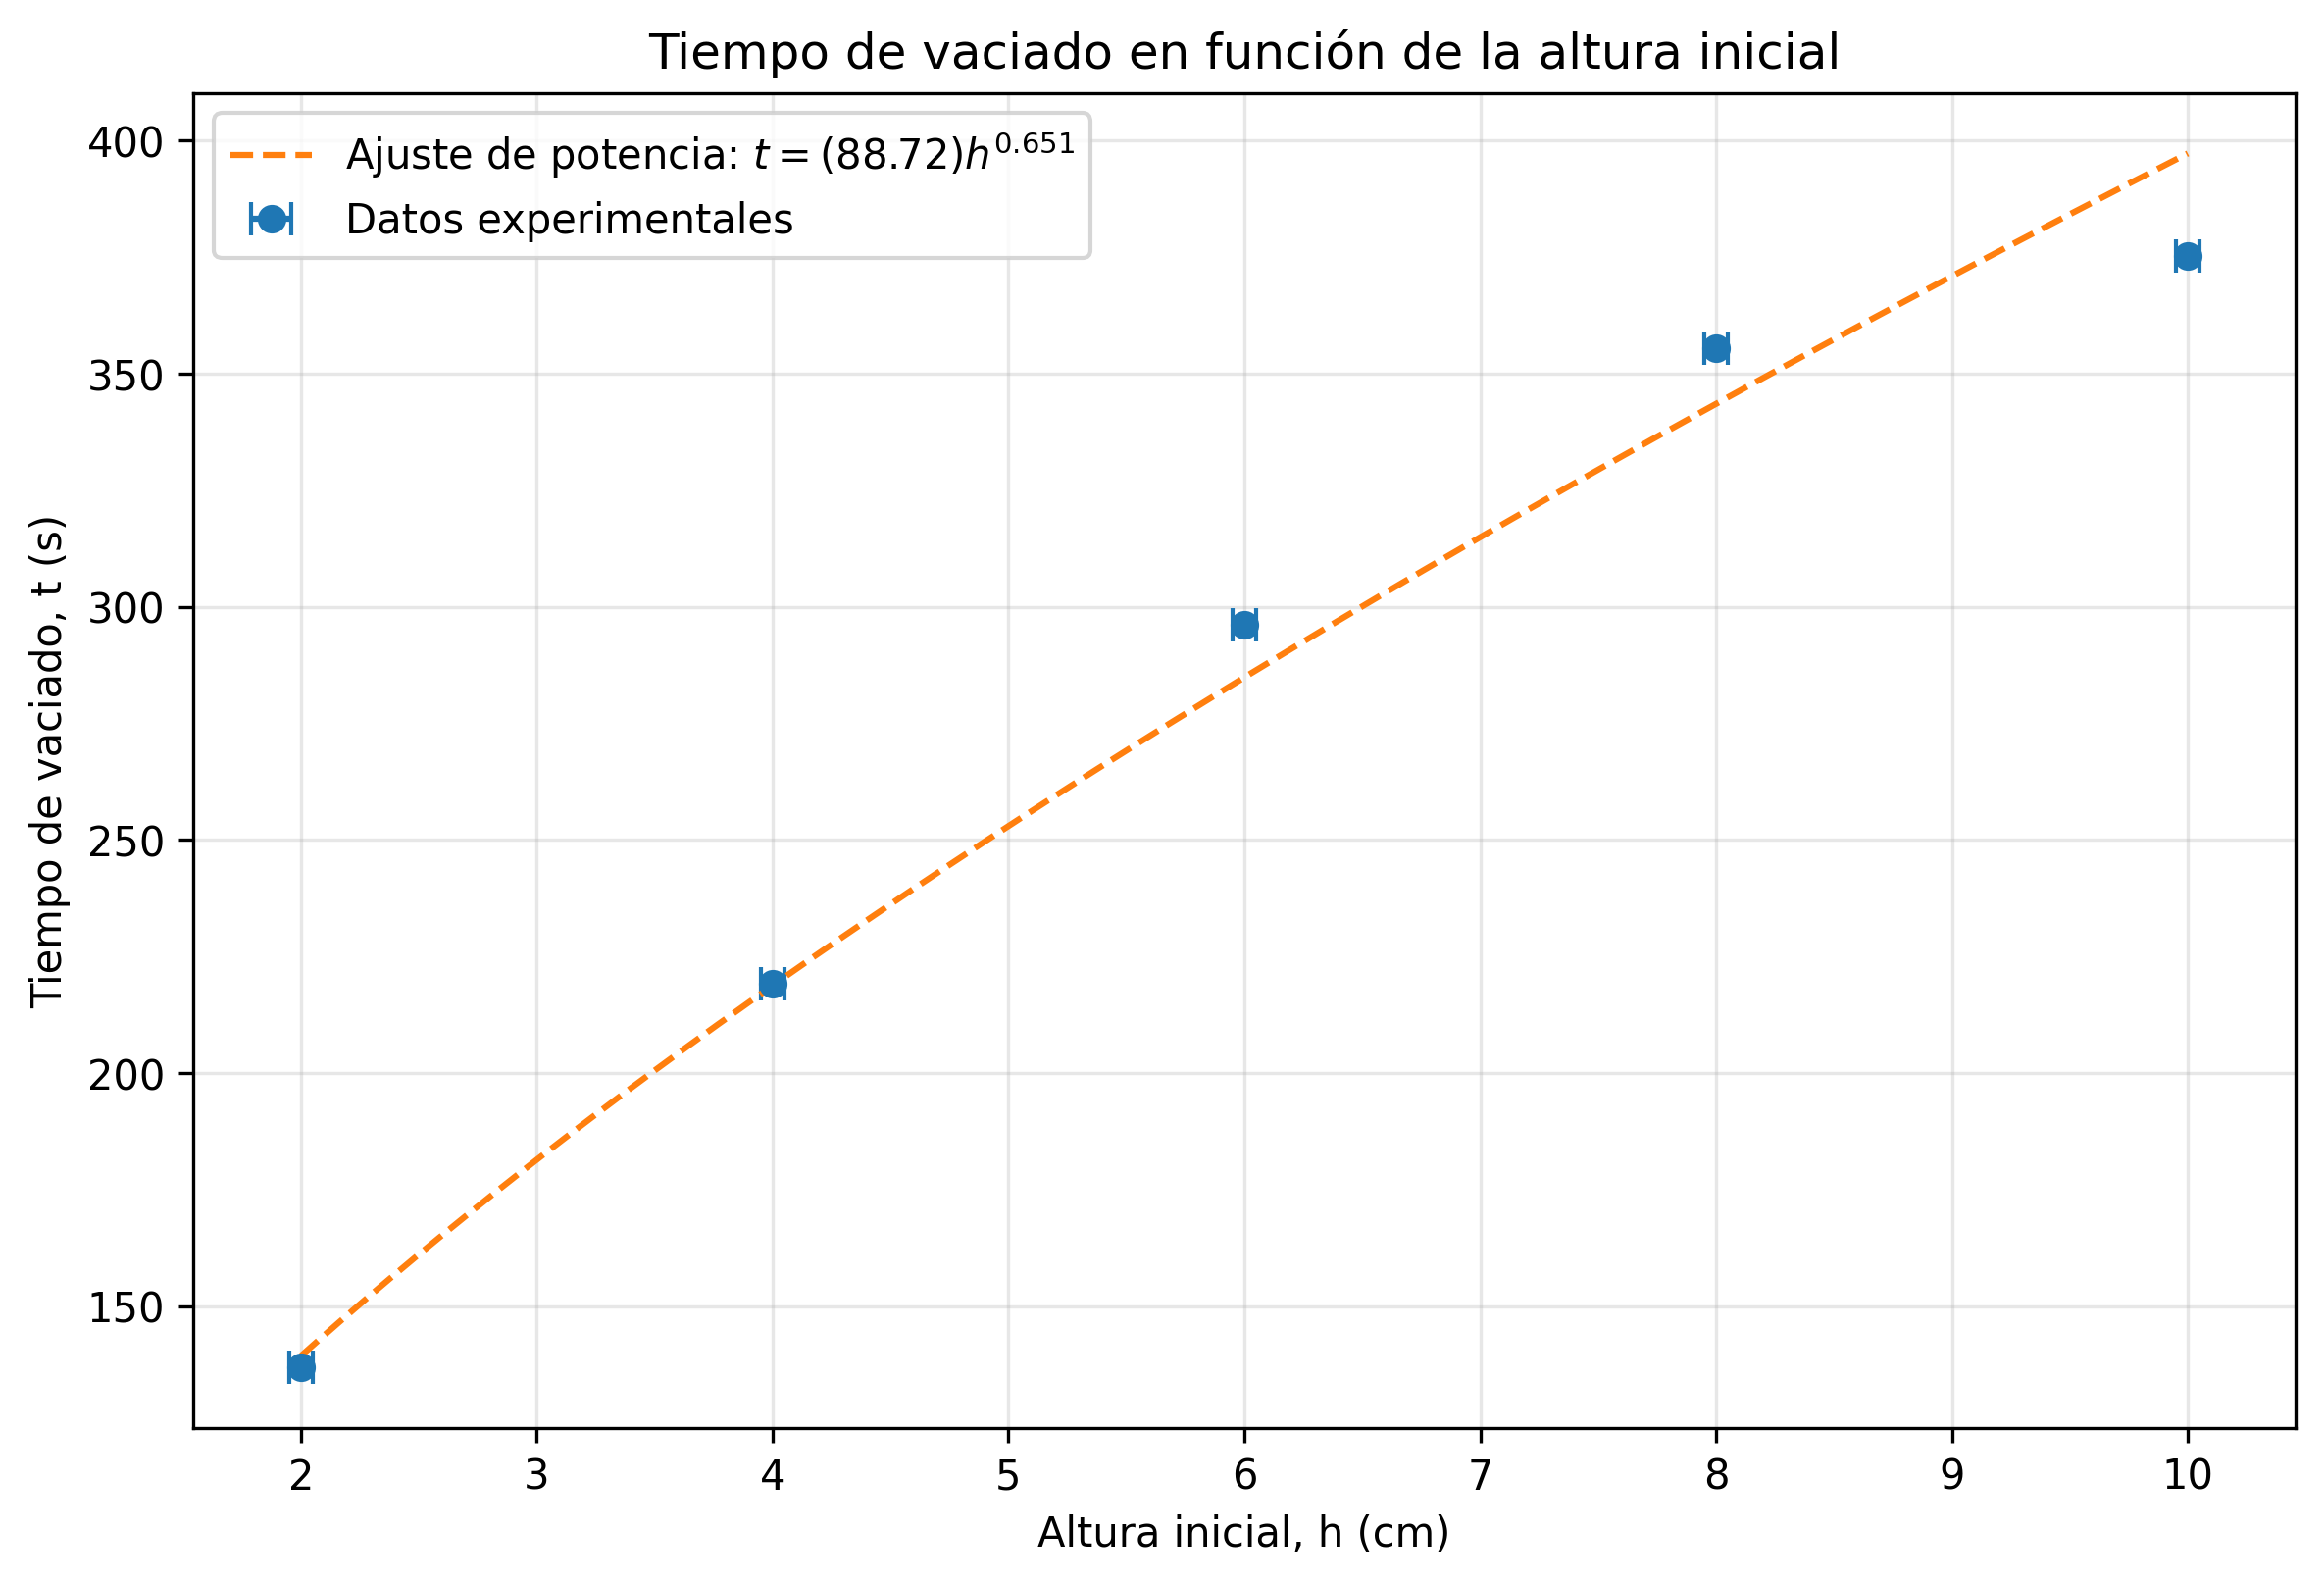
\includegraphics[width=0.85\linewidth]{images/grafica_t_vs_h_potencia.png}
\caption{Tiempo experimental de vaciado en función de la altura inicial. La línea representa el ajuste de potencia $t=(88.72)h^{0.651}$.}
\label{fig:potencia_torricelli}
\end{figure}

El exponente experimental obtenido, $n=0.651$, es menor que uno, lo que confirma que la relación entre el tiempo de vaciado y la altura inicial es sublineal. Sin embargo, este valor es mayor que el exponente teórico $n=0.5$ predicho por el teorema de Torricelli. 

Al comparar directamente los tiempos experimentales con los valores calculados mediante el modelo de Torricelli, se observa que el error porcentual fue de $15.64\%$, $22.48\%$, $17.81\%$, $11.60\%$ y $5.73\%$ para alturas de $10$, $8$, $6$, $4$ y $2\,\mathrm{cm}$, respectivamente. El error promedio de estas mediciones es aproximadamente $14.65\%$.

Los resultados muestran que el modelo de Torricelli reproduce adecuadamente la tendencia general de los datos, ya que tanto los valores experimentales como los teóricos indican que el tiempo de vaciado aumenta con la altura inicial de manera no lineal. 
No obstante, las diferencias entre ambos conjuntos de datos evidencian que el sistema experimental se aleja de las condiciones ideales del modelo.

Entre las posibles fuentes de error se encuentran el tiempo de reacción al utilizar el cronómetro manual, las incertidumbres en la medición de las alturas y diámetros. 

En conjunto, los resultados de esta segunda parte permiten verificar cualitativamente la dependencia sublineal esperada para el tiempo de vaciado. El ajuste experimental $t\propto h^{0.651}$ confirma que el tiempo no es directamente proporcional a $h$, mientras que la diferencia respecto al valor teórico $n=0.5$ evidencia las limitaciones experimentales y las aproximaciones utilizadas en el modelo de Torricelli.

\section{Discusión}

Interpretar el significado físico de los resultados y explicar si apoyan la hipótesis planteada. Analizar discrepancias entre teoría y experimento, limitaciones del procedimiento, fuentes de error sistemático y aleatorio, y el respaldo experimental de cada afirmación.

\section{Conclusiones}

Redactar conclusiones breves y fundamentadas en resultados cuantitativos. Indicar el cumplimiento de objetivos, la aceptación o rechazo de la hipótesis y mejoras concretas para trabajos futuros.

\section*{Agradecimientos}

Opcional. Incluir apoyo institucional, técnico o de laboratorio si corresponde.


\bibliographystyle{IEEEtran}
\bibliography{referencias}

\end{document}
